\chapter{Antennas, Sectors and Geometry}
\label{ch:antennas}

\begin{defbox}[In this chapter you will learn]
\begin{itemize}
 \item what antenna \emph{gain} really means and why it is measured in dBi;
 \item the 3GPP TR~38.901 horizontal sector pattern, including its half-power and floor behaviour;
 \item the geometric bookkeeping Amber performs: compass versus mathematical angles, bearings and angular error;
 \item how a three-sector base station divides the plane and how a node's ``best'' sector is chosen.
\end{itemize}
\end{defbox}

\section{Gain: concentrating a fixed amount of power}
\label{sec:gain}

An \emph{isotropic} radiator spreads power equally in all directions; its power
density at distance $d$ is $P_t/(4\pi d^2)$. No physical antenna is isotropic,
and the laws of energy conservation say that an antenna cannot create power, only
\emph{redistribute} it. A \emph{directional} antenna concentrates power into some
directions at the expense of others. Its \emph{gain} $G(\theta,\varphi)$ in a
direction is the ratio of the power density it produces there to that of an
isotropic radiator fed with the same power. We express it in \si{\dBi}.

\begin{intuition}[Gain as a flashlight]
Imagine pouring a fixed amount of light into a room. A bare bulb lights
everything dimly; a torch lights a narrow cone brightly and the rest not at all.
The brightness in the cone divided by the bare-bulb brightness is the gain. The
\emph{narrower} the beam, the \emph{higher} the gain---a fact we can quantify.
\end{intuition}

For a beam whose half-power widths are $\theta_{az}$ and $\theta_{el}$ (in
degrees) a standard approximation of the peak \emph{directivity} is
\begin{equation}
 D \;\approx\; \frac{41\,253}{\theta_{az}\,\theta_{el}},
\label{eq:directivity}
\end{equation}
because $41\,253\ \mathrm{deg}^2$ is the solid angle of the whole sphere in square
degrees. A cellular panel with a $65^\circ$ azimuth beamwidth and a vertical
beamwidth of roughly $10^\circ$ has $D\approx63\approx\SI{18}{dBi}$; losses
reduce this to the $\SI{15}{dBi}$--$\SI{17}{dBi}$ used in Amber's demos and in the
paper ($\SI{17}{dBi}$). A node's small antenna is nearly omnidirectional:
$\SI{0}{dBi}$ by default, $\SI{1}{dBi}$ in the paper's experiment.

\section{The 3GPP sector pattern}
\label{sec:patt3gpp}

Amber models a base-station sector with the \emph{horizontal} pattern of
3GPP TR~38.901 \citep{3gpp38901}. With $\varphi$ the angle between the target and the
antenna's boresight, $\varphi_{3\mathrm{dB}}$ the half-power beamwidth
(\codew{beamwidth_deg}) and $A_m$ the maximum attenuation (front-to-back
ratio), the attenuation below the peak is
\begin{equation}
 A_H(\varphi) \;=\; \min\!\left[\,12\left(\frac{\varphi}{\varphi_{3\mathrm{dB}}}\right)^{\!2},\; A_m\right]\ \mathrm{dB},
 \qquad
 G(\varphi) = G_{\max}-A_H(\varphi),
\label{eq:patt3gpp}
\end{equation}
with $A_m=\SI{30}{dB}$ as hard-wired in \codew{antenna_from_sector}.

\begin{figure}[t]
\centering
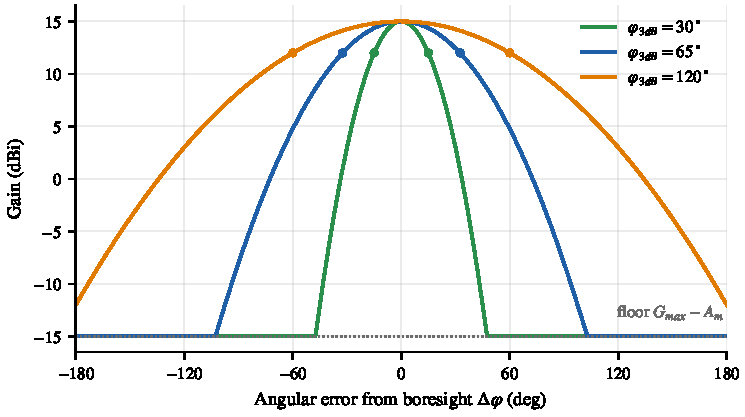
\includegraphics[width=0.85\linewidth]{fig_antenna}
\caption{The pattern of Eq.~\eqref{eq:patt3gpp} for $G_{\max}=\SI{15}{dBi}$ and three beamwidths. Dots mark the half-power points at $\pm\varphi_{3\mathrm{dB}}/2$ ($G_{\max}-\SI{3}{dB}$). Beyond about $1.58\,\varphi_{3\mathrm{dB}}$ the pattern is flat at $G_{\max}-A_m$.}
\label{fig:antenna}
\end{figure}

Three properties follow immediately and are worth internalising.
\begin{enumerate}
 \item \textbf{The half-power points.} At $\varphi=\varphi_{3\mathrm{dB}}/2$ the attenuation is
   $12\cdot\tfrac14=\SI{3}{dB}$. So $\varphi_{3\mathrm{dB}}$ is the \emph{full} width of the beam at
   half power---consistent with the name.
 \item \textbf{The floor.} The parabola reaches $A_m$ at
   $\varphi=\varphi_{3\mathrm{dB}}\sqrt{A_m/12}=1.58\,\varphi_{3\mathrm{dB}}$; for
   $65^\circ$ that is $102.8^\circ$. Beyond that the sector's gain is
   $G_{\max}-30$, i.e.\ $\SI{-15}{dBi}$ for a $\SI{15}{dBi}$ panel. The antenna
   never has a perfect null.
 \item \textbf{Narrow beams roll off fast.} A $30^\circ$ sector drops $\SI{12}{dB}$ at $\pm 30^\circ$,
   whereas a $65^\circ$ sector drops only about $\SI{2.6}{dB}$ there.
\end{enumerate}
We can check item~2 against the simulator. In the demo, \textbf{Node~0}
lies due north of the base station; the sectors at azimuths
$0^\circ,120^\circ,240^\circ$ see it at angular errors $0^\circ$, $120^\circ$ and
$120^\circ$. Sector~1 and~2 are therefore at the floor, $30$~dB below sector~0, and indeed
the simulator reports downlink powers of $+0.9$, $-29.1$ and $-29.1$~dBm for sectors
\code{BS0_S0}, \code{BS0_S1}, \code{BS0_S2}.

\begin{reality}[Only the azimuth cut is modelled]
The full 3GPP element pattern adds a \emph{vertical} term $A_V(\theta)$ and combines the two.
Amber implements the horizontal cut only (\codew{SectorAntenna3GPP.gain_linear}). The
base station's height enters path loss through the 3-D distance, but
\emph{there is no downtilt and no vertical attenuation}. For a node close to the mast
(a $\SI{20}{m}$ ground distance under a $\SI{25}{m}$ mast means the node is $\approx50^\circ$
below the horizon) a real panel would give less than the modelled gain.
\end{reality}

\section{Sectorisation}
\label{sec:sectorisation}

A cell site rarely uses a single omnidirectional antenna. The usual
arrangement is \emph{three sectors of $120^\circ$ spacing}, each with a
directional panel. This multiplies capacity (each sector reuses the spectrum)
and, for a given transmit power, lifts the gain in each served direction.

Because the sector pattern falls off by about $\SI{10}{dB}$ at the
crossover ($60^\circ$ off boresight when sectors are spaced $120^\circ$ apart),
a $65^\circ$ panel leaves a \emph{ripple} in the coverage:
\[
 G(60^\circ)=15-12\left(\tfrac{60}{65}\right)^{2}=\SI{4.8}{dBi},
\]
more than $\SI{10}{dB}$ below the peak. This ripple is visible as the darker
bands between sectors in coverage maps such as Figure~\ref{fig:covmap}.

\begin{figure}[t]
\centering
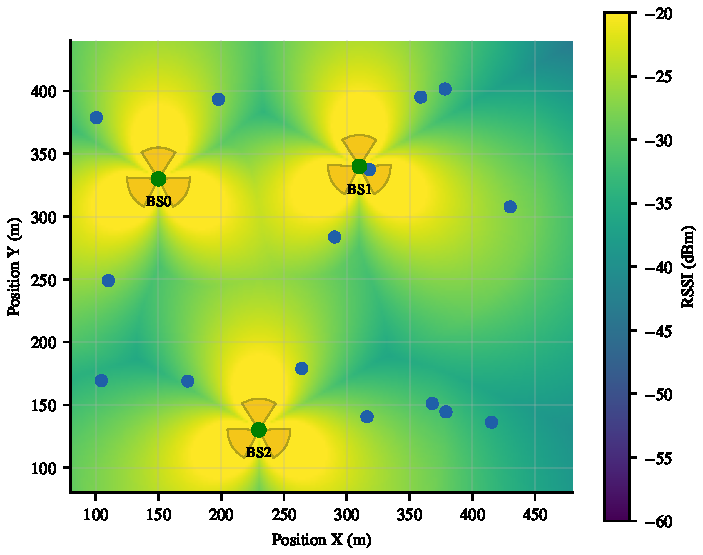
\includegraphics[width=0.6\linewidth]{fig_coverage}
\caption{A coverage map produced by Amber's \code{CoverageMap} for an illustrative deployment (three base stations of three $65^\circ$ sectors, $\SI{30}{dBm}$, $\SI{17}{dBi}$, $\SI{924}{MHz}$, 15 random nodes), in the style of the paper's Figure~1. Colour is the \emph{best} received power among all sectors (Chapter~\ref{ch:coverage}). This figure is our own example, not the paper's data.}
\label{fig:covmap}
\end{figure}

\paragraph{The best sector.}
Amber assigns each point (grid point or node) to the sector delivering the
highest power: the ``owner'' of that point (\code{owner}, \code{best_pw_dbm}). There is
no hysteresis or handover logic, and ties are resolved in favour of the sector
evaluated first (the comparison is a strict ``$>$'').

\section{Geometry: bearings and angular errors}
\label{sec:geometry}

To evaluate Eq.~\eqref{eq:patt3gpp} we need $\varphi$, the angle between a
sector's boresight and the direction to a node. Two angle conventions meet here, and
confusing them is a classic source of bugs.
\begin{itemize}
 \item \textbf{Compass} (navigation) azimuth: $0^\circ$ is North, increasing \emph{clockwise}.
   This is what \codew{Sector.azimuth_deg} and \codew{Node.azimuth_deg} use.
 \item \textbf{Mathematical} angle: $0^\circ$ is East, increasing \emph{counter-clockwise}.
   This is what \codew{numpy.arctan2} returns.
\end{itemize}
The conversion is $\theta_{\mathrm{math}}=(90^\circ-\alpha_{\mathrm{compass}})\bmod360^\circ$
(\codew{compass_to_math}). The bearing from a point $(x_0,y_0)$ to $(x,y)$ is
$\operatorname{atan2}(y-y_0,\,x-x_0)\bmod360^\circ$ (\code{bearing_deg}), and the
smallest angular difference between two angles, correct across the $0^\circ/360^\circ$ seam, is
\begin{equation}
 \Delta\varphi=\left|\,(\theta_{\mathrm{target}}-\theta_{\mathrm{bore}}+180^\circ)\bmod360^\circ-180^\circ\,\right|
\label{eq:angerr}
\end{equation}
(\codew{angular_error_deg}). The shift by $180^\circ$ followed by the modulus maps the
difference into $[-180^\circ,180^\circ)$, whose absolute value is the shortest
way round.

\begin{figure}[t]
\centering
\begin{tikzpicture}[scale=1.05]
 \fill[ablue!14] (0,0) -- (27.5:3.0) arc (27.5:92.5:3.0) -- cycle;
 \draw[->,agrey] (-1.2,0) -- (4.3,0) node[right,lab,align=left] {East\\math $0^\circ$};
 \draw[->,agrey] (0,-1.0) -- (0,3.6) node[above,lab,align=center] {North, compass $0^\circ$};
 \draw[->,very thick,ablue] (0,0) -- (60:3.4) node[above right,lab,align=left] {boresight\\compass $30^\circ$\\math $60^\circ$};
 \draw[->,thick,agreen] (0,0) -- (12:3.9) node[right,lab,align=left] {target bearing\\math $12^\circ$};
 \draw[ablue] (1.0,0) arc (0:60:1.0);
 \node[lab,ablue] at (1.35,0.35) {$\theta_{\mathrm{bore}}=60^\circ$};
 \draw[aorange] (0,1.6) arc (90:60:1.6);
 \node[lab,aorange,anchor=south west] at (0.35,1.7) {$\alpha=30^\circ$};
 \draw[ared,thick] (2.6,0.56) arc (12:60:2.65);
 \node[lab,ared,anchor=west] at (2.85,1.55) {$\Delta\varphi=48^\circ$};
\end{tikzpicture}
\caption{Compass versus mathematical angles. The sector's boresight points at compass azimuth $30^\circ$ (math $60^\circ$); a target at math bearing $12^\circ$ is $\Delta\varphi=48^\circ$ off boresight and sees the pattern attenuation $12(48/65)^2=\SI{6.5}{dB}$ for a $65^\circ$ sector.}
\label{fig:angles}
\end{figure}

\begin{example}[Why a node due north sees the $120^\circ$ sector at the floor]
The sector with compass azimuth $120^\circ$ has $\theta_{\mathrm{bore}}=(90-120)\bmod360=330^\circ$.
A node due north has math bearing $90^\circ$. By Eq.~\eqref{eq:angerr}:
$\left|(90-330+180)\bmod 360-180\right|=\left|300-180\right|=120^\circ$, and
$12(120/65)^2=40.9>A_m$, so the attenuation clips at $\SI{30}{dB}$.
\end{example}

\section{Node antennas and reciprocity}

A node is described by \codew{antenna_type}: ``omni'' (default; gain
\codew{antenna_gain_dbi}, independent of direction) or ``3GPP'' (the same pattern as a
sector, with the node's own \code{azimuth_deg} and \codew{beamwidth_deg}).
In both the downlink and the uplink the simulator evaluates the node's gain
toward the base station \emph{with the same function}. This reflects the
\emph{reciprocity} of passive antennas: the pattern is the same in transmit and
receive. For backscatter, where one antenna both receives the carrier and
re-radiates the reflection, reciprocity is physically exact.

\begin{codemap}
\small
\begin{tabularx}{\linewidth}{@{}>{\ttfamily}p{5.0cm}X@{}}
\toprule
\normalfont\bfseries Concept & \normalfont\bfseries Code (\file{amber/propagation.py})\\
\midrule
Pattern Eq.~\eqref{eq:patt3gpp} & \codew{SectorAntenna3GPP.gain_linear}\\
Omni antenna & \codew{OmniAntenna.gain_linear}\\
Build antenna from device & \codew{antenna_from_sector}, \codew{antenna_from_node}\\
Compass $\to$ math & \codew{compass_to_math}\\
Bearing, error Eq.~\eqref{eq:angerr} & \code{bearing_deg}, \codew{angular_error_deg}\\
Best sector & the \codew{mask = p_w > best_pw_w} update in \codew{compute_bs_to_point}\\
\bottomrule
\end{tabularx}
\end{codemap}

\section{Chapter summary}
\begin{itemize}
 \item Gain redistributes power; narrower beams have higher gain, $D\approx41\,253/(\theta_{az}\theta_{el})$.
 \item Amber uses 3GPP's horizontal pattern: $G=G_{\max}-\min[12(\varphi/\varphi_{3\mathrm{dB}})^2,30]$.
 \item Three $65^\circ$ sectors at $120^\circ$ spacing leave a $\approx10$~dB ripple at the crossovers.
 \item Compass and mathematical angles differ; Eq.~\eqref{eq:angerr} gives the correct shortest angular error.
 \item No vertical pattern or downtilt is modelled.
\end{itemize}

\section*{Exercises}
\begin{exercise}
A sector has $G_{\max}=\SI{17}{dBi}$ and $\varphi_{3\mathrm{dB}}=65^\circ$. What is its gain at an angular error of $40^\circ$? At $90^\circ$? At $150^\circ$?
\end{exercise}
\begin{exercise}
Find the angular error at which the pattern reaches its floor for (a) $\varphi_{3\mathrm{dB}}=30^\circ$ and (b) $\varphi_{3\mathrm{dB}}=120^\circ$.
\end{exercise}
\begin{exercise}
Convert the compass azimuths $0^\circ$, $45^\circ$, $135^\circ$, $270^\circ$ to mathematical angles. A sector has compass azimuth $10^\circ$; a node is at math bearing $350^\circ$. What is the angular error?
\end{exercise}
\begin{exercise}
Three sectors with $\varphi_{3\mathrm{dB}}=65^\circ$ at compass azimuths $0^\circ,120^\circ,240^\circ$. For a node at compass bearing $60^\circ$ from the mast, compute each sector's gain (take $G_{\max}=\SI{15}{dBi}$) and say which sector Amber would call the owner.
\end{exercise}
\begin{exercise}
Estimate the peak gain of a panel with a $90^\circ\times15^\circ$ beam using Eq.~\eqref{eq:directivity}.
\end{exercise}
